\documentclass[]{llncs}

\usepackage{graphicx}
\usepackage{float}
\usepackage{url}
\usepackage{fancyhdr}
\pagestyle{fancy}
\lhead{}
\chead{}
\rhead{Implementation OPC UA on Secure Device}
\lfoot{}
\cfoot{}
\rfoot{\thepage}
\renewcommand{\headrulewidth}{0.4pt}
\renewcommand{\footrulewidth}{0.4pt}
\RequirePackage{filecontents}

\begin{document}
\title{Implementation Object Linking and Embedding for Processes Control Unified Architecture Specification on Secure Device} %titles have no end punctuation
\author{Yuankui Wang (Matr.-Nr.: 6670785)}
\institute{University of Paderborn \email{wangyk@mail.upb.de}}

\maketitle

\begin{abstract}

Object Linking and Embedding for Process Control Unified Architecture, known as OPC UA is the most recent released industry standard from OPC Foundation, which compared with his predecessors is equipped with a list of charming new features, with whose help OPC UA is capable of developing a common communication interface for devices which participate in automation system.Meanwhile, the technology of smart card is widely used in information security fields of finance, communication, personal and government identification, payment. Therefore it is meaningful and promising to develop OPC UA standard compliant application on embedded smart card secure device, for the purpose of secure remote control, enterprise resource planning and etc. Since the storage and compute capacity of chip card is limited, OPC UA product will consist of two essential parts, namely client/server application code, realized as Android or other application, and communication stack, realized as Javacard Applet based on Remote Application Management from GlobalPlatform. The implemented demonstration scenarios and corresponding analysis show the possibility of developing OPC UA standard compliant application on devices embedded with smart card to benefit customers. 
\end{abstract}

\section{Introduction and Motivation}

According to the \emph{Mobile Economy 2013} from \emph{Global System for Mobile Communications Association}, at the end of year 2013 there are over 3.2 billion mobile   subscribers in total, which means one half the population of the earth now enjoy the social and economic convenience brought by mobile technology. Moreover by year 2017 700 million new subscribers are expected to be added. And the number of mobile subscriber will reach 4 billion in 2018. Mobil technology opens nowadays a promising market. 

Mobile products  play an irreplaceable role at the heart of our  daily life. With the help of mobile technology, the user's world in many domains such as, education, financial transactions, health and etc. are inter-connected. Mobile users are enjoying the advantages of mobility. Services, like 24/7 monitored home security, full control about the management of home humidity and temperature, exist not only in science fiction film but also could be realized by today's technology.

At the same time, mobility in industry and business world is also a critical  assert, which can not only increase efficiency and productivity but also drive new revenue generation and competitive advantage. The most convicting example here is Machine to Machine communication, that is also referred as M2M technology. In M2M communication, machines which are usually embedded with smart cards exchange gathered date with each other to accomplish common task using wireless or wired networks. M2M technology is widely employed in different industry spheres such as factory automation, remote access control and sensor monitoring. It boosts the efficiency of corresponding processes, offers centralized service support and date management, minimizes system response time.

But in order to enjoy the aforementioned features, two tough issues must be resolved. First, how to achieve a common interface for the devices that participate in the system.  And second how to guarantee system security under different communication environments with various date complexity.

\subsection{Solution Idea}
In this master thesis, I am going to address solutions for questions mentioned in  section \emph{Introduction and Motivation} and  design a smart home system for the purpose of demonstration. In this smart home system, home owner using smart phone is capable of experiencing 24/7 home security service, remotely managing inner home environment parameters and assigning access permissions. This system consists of smart phones with Universal Integrated Circuit Cards (UICC  smart card), digital door locks, control devices and environment sensors. Moreover each device is equipped with smart card, which acts not only as secure token, that saves  user credentials, but also is in charge of communication management with other device.

In particular, I will introduce the newly released industry automation standards object linking and embedding for processes control unified architecture(OPC UA standards) to build a common communication interface for devices that are mentioned above and design a OPC UA specification compliant communication stack on UICC smart card., whose duties are: creation and management communication between OPC client/server application, entity authentication and secure message exchange.

\subsection{Paper Structure}
At first, in the second chapter I will present the fundamental technologies which will be frequently mentioned in this paper. Secondly the state of art, for instances mobile security,  home remote control technologies, Remote Application Management from GlobalPlatform will be introduced, which act together as cornerstone for my implementation scenario. In the fourth section, I am going to focus on  UICC mobile security  and base on UICC framework build a  OPC UA standards scarifying communication stack  as Javacard Applet with the help of GlobalPlatform  specifications. In the next implementation chapter, I will present how my  demonstration scenario can be realized. As sixth and seventh chapter,  test and performance analysis will be describe to show the reliability and security of my proposal.
  
\section{Fundamental Technologies}
In this section, i am going to give a brief introduction about technologies and terminologies that are applied in this paper. 

\subsection{OPC Unified Architecture Structure Overview }
Object Linking and Embedding for Process Control Unified Architecture, known as OPC UA is the most recent released industry standards from OPC Foundation, acts nowadays as the most promising candidate in industry M2M automation world, whose major duty is the build a secure communication interface for machines that participate in automation system. 

\subsubsection{OPC UA Specifications}

The whole OPC Unified Architecture specification can be divided into three main parts, core specification part, which consists of OPC UA concepts, security model, address space model, services, information model, service mapping and profiles, access type specification part including date access, alarm and conditions, programs and historical access, at last utility specification part covering discovery together with aggregates.
\begin{table}[!htbp]
\caption{OPC UA specifications}
\centering
\begin{tabular}{ c c }
\hline\hline
OPC UA Part1 &Overview and Concepts Specification \\
OPC UA Part2 &Security Model Specification \\
OPC UA Part3 &Address Space Model Specification\\
OPC UA Part4 &Services Specification\\
OPC UA Part5 &Information Model Specification  \\
OPC UA Part6 &Mappings Specification \\
OPC UA Part7 &Profiles Specification \\
OPC UA Part8 &Data Access Specification  \\
OPC UA Part9 &Alarms and Conditions Specification \\
OPC UA Part10 &Programs Specification  \\
OPC UA Part11 &Historical Access Specification \\
OPC UA Part12 &Discovery and Aggregates Specification \\
\hline
\end{tabular}
\label{table:opcua}
\end{table}

\subsubsection{OPC UA Client Server Structure}
 OPC UA standards apply the classic client server architecture, where server is in charge of managing functionalities and data information on a machine device, for instance temperature data gathered by  a remotely allocated sensor. Meanwhile client possesses the ability to query information from server, submit subscription and send command to server.

\begin{figure}[!htbp]
	\centering
	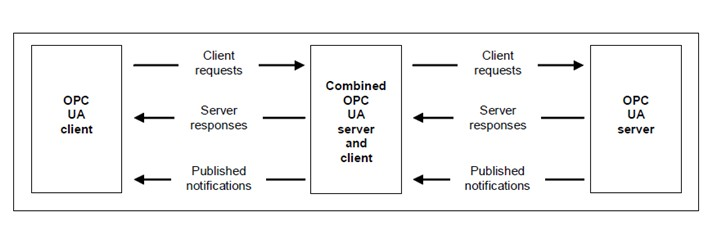
\includegraphics[width=1.00\textwidth]{cs.jpg}
		\caption[ ]{OPC UA Client Server Structure\cite{O1}}
	\label{fig:cs}
\end{figure}
Figure~\ref{fig:cs} illustrates a typical OPC UA client server architecture and also describes an internal combined server-client structure. The routine communication between client and server consists of requests from client, corresponding responses sent by server and notifications which are generated because of client's early subscription.

\subsubsection{OPC UA Terminologies}
In OPC Unified Architecture on server stored information that can be visited by clients is defined as \emph{address space}\cite{O3} and there also exits a set of services\cite{O4} which are provided by server and are introduced in order to apply operations on \emph{address space}. Information in address space is organized as a set of in particular hierarchy structured \emph{Objects}. \emph{Object} here could refer to data gathered by sensor, server system parameters and etc. Clients can query and accept information provided by OPC Unified Architecture Servers in two major ways, \emph{binary structured data} and \emph{XML documents}, depending on the complexity of exchanged date, network quality and so on. In addition three kinds of transport protocol are already defined to support client server communication. They are: \emph{OPC UA TCP}, \emph{HTTP/SOAP} and \emph{HTTP}. Also the hierarchy structure in which \emph{Objects} are organized in \emph{address space} is also various and not only limited to simple single hierarchy.   

One of the charming features provided by OPC UA is \emph{Event Notifications}. With the help of \emph{Event Notification}, OPC UA servers are allowed immediately after satisfaction of conditions, which is normally predefined by a client, to publish data to particular client. In this way, clients can for instance discovery failures within client-server-communication quickly and recover that communication as soon as possible, which in return minimizes the lost to the smallest possible amount. Also clients are able to observe the subscribed data more precisely and find the pink elephant as fast as possible.

\subsubsection{Standard OPC UA Server}
\begin{figure}[!htbp]
	\centering
	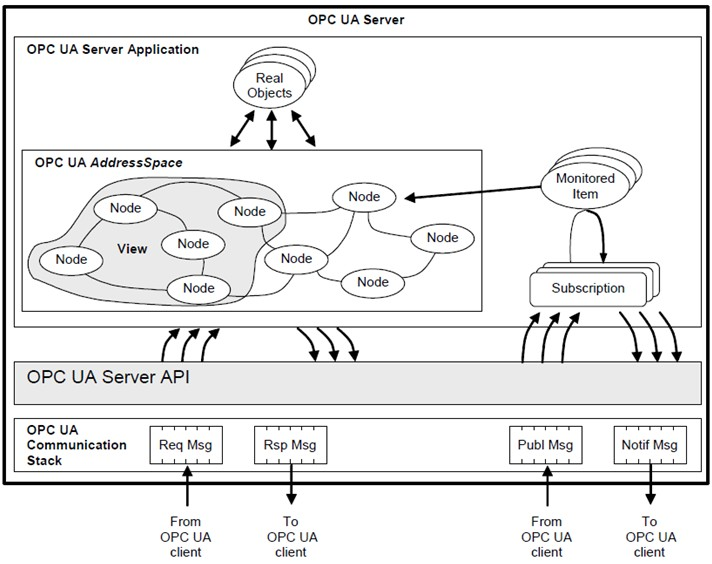
\includegraphics[width=1\textwidth]{server.jpg}
		\caption[ ]{OPC UA Server Structure\cite{O1}}
	\label{fig:server}
\end{figure}
In figure~\ref{fig:server}, the structure of one standard OPC UA Server is described. It includes three main parts, server application, internal API and communication stack. In server application part,  functionalities and services which are offered by OPC UA standards are realized, such as \emph{Event Notification} , processing request from connected OPC UA client, data encryption and decryption. Moreover, \emph{Real objects}  here  refers physical field devices and software applications that are maintained and managed by OPC UA server. \emph{Nodes} in \emph{Address Space} presents  abstractly above mentioned \emph{Real Ojbects}. \emph{View}, which is pictured as a part of address space, presents \emph{Objects} that can be browsed by particular clients. The main  task for communication stack  is to establish communication session based on secure channel between OPC UA client and server. Typically communication messages which are exchanged frequently among clients and servers are, request-, notification- message from client and   corresponding   response-, publish message from server. At last, an internal API connects the server application and the communication stack.

\subsubsection{Standard OPC UA Client}
\begin{figure}[!htbp]
	\centering
	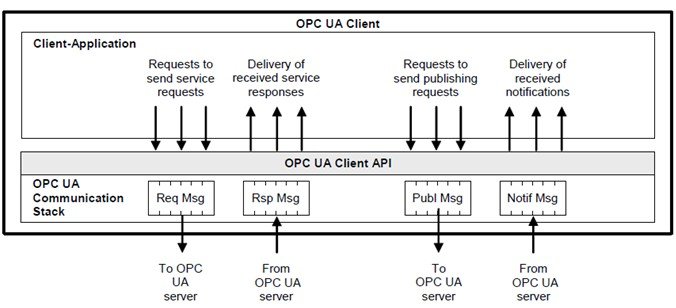
\includegraphics[width=1.1\textwidth]{client.jpg}
		\caption[ ]{OPC UA Client Structure\cite{O1}}
	\label{fig:client}
\end{figure}

Figure~\ref{fig:client} pictures one simple OPC UA client containing client application, an internal API, isolating the application code from communication stack, and a communication stack that converts API calls into messages and delivers them to OPC UA server.

\subsubsection{Secure Channel and Session}

\begin{figure}[!htbp]
	\centering
	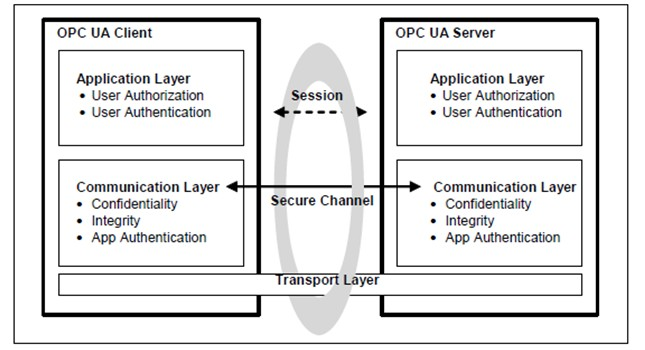
\includegraphics[width=0.95\textwidth]{opc_ua_cs_comm.jpg}
		\caption[ ]{OPC UA Client Server Communication\cite{O2}}
	\label{fig:opc_ua_cs_comm}
\end{figure}

Since some data exchanged between client and server could be extreme precious and should be protected from other malicious third party, OPC UA defines a full set of  \emph{security model}, with which sytem developer can configure the security level of the application to meet the need of reality. In the \emph{security model}, authentication of client and server, authorization, integrity and confidentiality of client-server-communication, auditability(also known as traceability ) and availability of services are guaranteed. Also OPC UA  standard provides a set of countermeasures against attacks such as message flooding, eavesdropping, message spoofing, message alteration, message reply, server profiling, session hijacking and so on\cite{O2}.


Figure~\ref{fig:opc_ua_cs_comm} pictures the typical communication architecture between OPC UA client and server. As shown in~\ref{fig:opc_ua_cs_comm}, the communication between OPC UA client and server is established above a secure channel, which is active during the whole application session and in this session, the state information, such as algorithms used for authentication, user credentials, is maintained. The secure channel is established only after successful validation of both client and server certificates and it provides necessary mechanisms to support confidentiality, message integrity and application authentication. On top of secure channel, is an application level session between OPC UA client and server, whose responsibility is to transmit data information and commands. It should be pointed out that, even a secure channel is out of work for some reasons, the session is still valid and OPC UA client and server involved in aforementioned session can still re-establish the broken secure channel. A secure transport layer is guaranteed by encryption and signatures methods provided by platform that supports OPC UA structure.

\begin{figure}[!htbp]
	\centering
	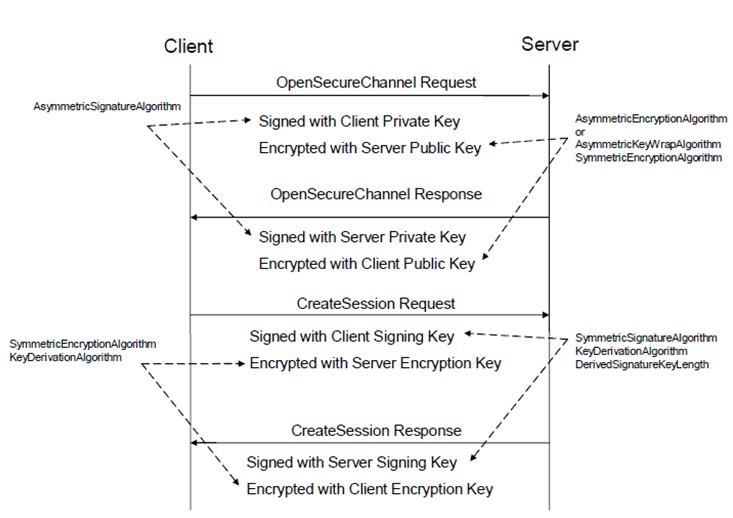
\includegraphics[width=1\textwidth]{opc_ua_shs.jpg}
		\caption[ ]{OPC UA Client Server Security Handshake\cite{O2}}
	\label{fig:opc_ua_cs_shs}
\end{figure}
\subsubsection{Security Handshake}
Security handshake as below explains with some details how secure channel and session are established. Normally OPC UA client initiates the first \emph{OpenSecureChannel} request and waits the response from server. Messages exchanged during the process of construction secure channel between client and server are encrypted using asymmetric encryption and signature algorithms. But some security protocols that could be applied according to OPC UA standard, are not using an asymmetric message encryption algorithm to encrypt to request/response messages. Instead, they apply AsymmetricKeyWrapAlgorithm to encrypt symmetric keys and use symmetric encryption algorithm with encrypted keys to encrypt messages. After a successful construction of secure channel, OPC UA client sends \emph{CreateSession} request and waits for server response. Messages transported during this procedure are encrypted with symmetric encryption algorithms and signed with client/server signing key.
\begin{figure}[!htbp]
	\centering
	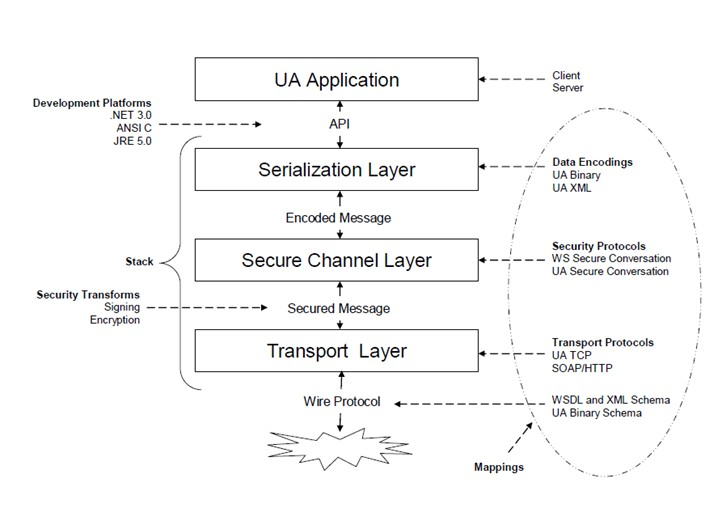
\includegraphics[width=1\textwidth]{opc_ua_commstack.jpg}
		\caption[ ]{OPC UA Client Server Communication Stack\cite{O2}}
	\label{fig:opc_ua_commstack}
\end{figure}

\subsubsection{OPC UA Communication stack}
As described in figure~\ref{fig:opc_ua_commstack}, according to different responsibility, OPC UA communication stack consists of three parts: application layer, communication layer and transport layer. Even the terminologies of those layers using the same English words as the ones used in ISO model, but they are not equal to layers in ISO model. Figure~\ref{fig:opc_ua_commstack} also pictures a precise functionality overview of each component.

UA Application part realizes client or server application. Serialization layer together with secure channel layer build the communication layer and their job is dividing long message into pieces referred as message chunk, encrypting each individual message chunk and forwarding encrypted message chunk to transport layer. When receiving message chunk from others, OPC UA message receiver firstly verifies whether this message piece meets the security standard negotiated between OPC UA client and server. If not, message receiver will close the secure channel. After a successful verification of all message chunks, the original OPC UA message will be reconstructed and sent to UA Application Code through API. Each secure message chunk applies the following structure described in figure~\ref{fig:opc_ua_messchunk}.

Knowing the essential parts of OPC UA communication stack, in the following subsections the establishment, re-establishment and close of communication channel are explained.

\begin{figure}[!htbp]
	\centering
	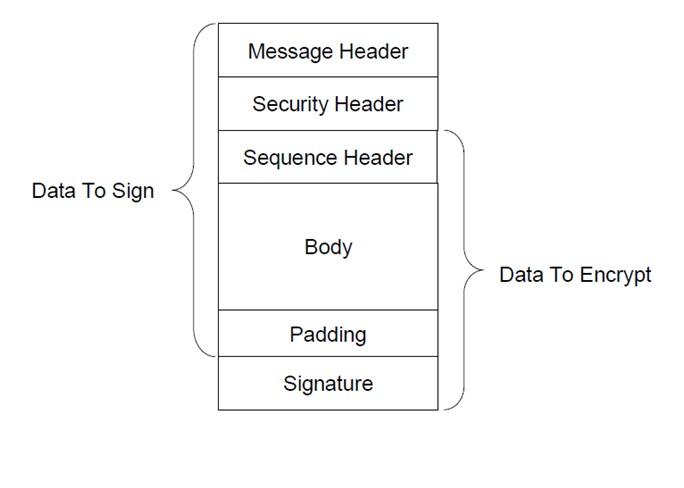
\includegraphics[width=0.75\textwidth]{opc_ua_messchunk.jpg}
		\caption[ ]{Message Chunk Structure\cite{O2}}
	\label{fig:opc_ua_messchunk}
\end{figure}

\begin{figure}[!htbp]
	\centering
	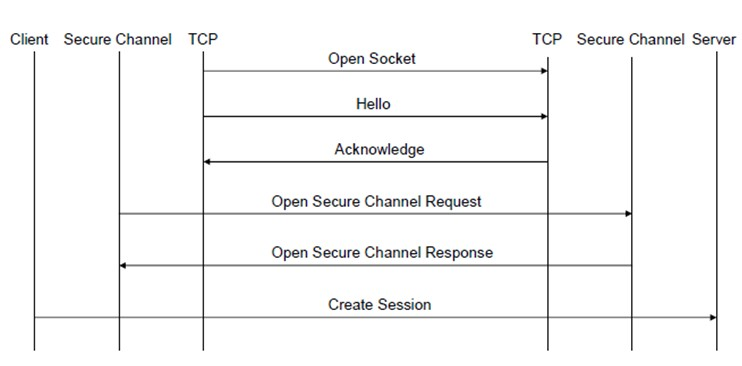
\includegraphics[width=1\textwidth]{tcp_1.jpg}
		\caption[ ]{Establish TCP/IP Connection\cite{O6}}
	\label{fig:tcp_1}
\end{figure}

\paragraph{Establishment of communication channel}
As the first step to create TCP/IP connection, this process is normally initialized by OPC UA client. OPC UA client initiates his socket and sends \emph{helloMessage}, that includes supported buffer size which specifies the message chunk size used for future communication, to the target OPC UA server. After receiving greeting message, OPC UA server answers the request for establishing TCP/IP connection with acknowledge message and reports suggested buffer size to his own secure channel layer. Moreover during the creation of communication channel, the greeting \emph{hallo} and answering \emph{acknowledgment} messages could only be sent once. If OPC UA client or server receives more than one above-mentioned message from a same sender, error will be reported and corresponding communication socket will be closed.
\begin{figure}[!htbp]
	\centering
	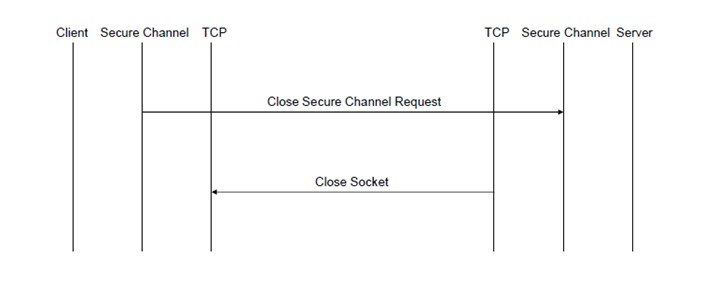
\includegraphics[width=1\textwidth]{tcp_2.jpg}
		\caption[ ]{Close TCP/IP Connection\cite{O6}}
	\label{fig:tcp_2}
\end{figure}
\paragraph{Close TCP/IP Connection}
This process is done when OPC UA server receives \emph{CloseSecureChannel} request from OPC UA client. During this process, server releases all the resource taken by corresponding secure channel and sends none response.
\begin{figure}[!htbp]
	\centering
	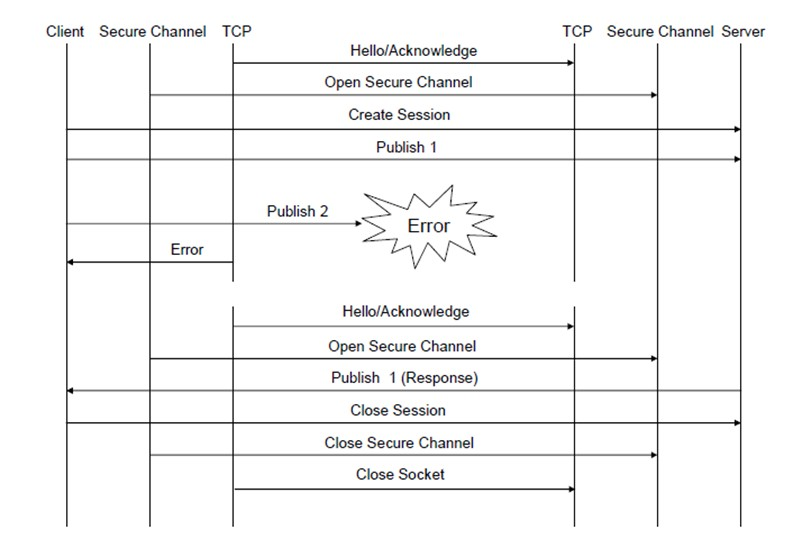
\includegraphics[width=1\textwidth]{tcp_3.jpg}
		\caption[ ]{Recover Secure Channel\cite{O6}}
	\label{fig:tcp_3}
\end{figure}

\paragraph{Recover Secure Channel}


Whenever error occurs during TCP/IP connection between OPC UA client and server, client will try to periodically re-establish it until the session is closed or the lifetime of security token goes to an end. Also it should be pointed out that the buffer size defined by corrupt secure channel should not be changed during this error recover process.

\subsubsection{Historical Data}
Last but not least security feature offered by OPC Unified Architecture is auditing, which supports traceability of any behaviours occur in OPC UA system. This record can be used for forensic research.


\subsubsection{Other Competitor}
WebSphere Message Broker Message Queuing Telemetry Transport (MQTT)\cite{Ref3} is another machine to machine (M2M) communication protocol. Compared with OPC UA standard, MQTT also supports UDP protocol in the transport layer. In OPC UA, only unidirectional, client to server, communication is provided, but in MQTT server to client communication is also possible without server implements client code. Moreover the communication overhead of MQTT is in comparison with OPC UA is relative small. 


Even thought MQTT protocol supports communication environment with low bandwidth and high latency, OPC UA provides complex object model and supports more features, including historical data record, alarm, notification, complete security policies and this is reason why OPC UA is more suitable for the application scenario that handles sensitive data with complex structure and needs immediate response.


Another member from Internet of Things is Constrained Application Protocol (CoAP)\cite{Ref5} which is designed for the extreme simple electronic devices with less memory and computing power and original CoAP only runs over UDP. Compared with OPC UA, simplicity from CoAP is the advantage, but apparently it should be considered that in the implementation scenario other transport protocol could be used, like TCP, more functions and services other than pure message exchange between client and server, are requested from users.

\subsection{UICC}
The Universal Integrated Circuit Card is the smart card used in mobile terminals in GSM and UMTS networks. It enables authenticated subscriber to join the network with their mobile terminals and at the same time protects essential user data. UICC acts  also most time as the secure token, which stores and protects subscriber's confidential information. Moreover, as a 32bit processor, UICC is also capable of processing necessary  encryption and  decryption algorithms\cite{uiccDef}.

\subsubsection{Smart Card}
Smart Card, whose characteristic feature is an integrated circuit that is embedded in a chip card, which is capable of performing data process, information storage and message transmitting\cite{handbuch}. The most charming feature of smart card is that, sensitive user's credential data such as certificates, encryption keys, digital signature along with other precious user information can only be accessed though a serial interface, which stands under  strict control of the card operation system. This characteristic provides strong  protection against  unauthorized data access and ensures the confidentiality of on card stored information. Therefor smart cards are widely used in applications that require strong protection.

With sophisticated communication protocol using Application Protocol Data Units(APDU), smart card and Card Accepting Device(CAD) are able to process secure message exchange. Smart card is also able to process cryptographic algorithms on hardware. Nowadays, it supports symmetric key algorithms like DES, triple DES; standard public key cryptography for instance RSA, hash functions such as commonly SHA-1\cite{handbuch}. More powerful microprocessor on chip card is, the speed performance is better.  

\begin{table}[ht]
\caption{ISO/IEC 7816\cite{handbuch}}
\centering
\begin{tabular}{ c c }
 ISO7816 document & Description  \\[1ex]
\hline\hline
 ISO 7816-1&Physical characteristics   \\
ISO 7816-2&Dimensions and location of the contacts   \\
 ISO 7816-3& Electronic signals and transmission protocols   \\
ISO 7816-4&Industry commands for interchange  \\
ISO 7816-5& Number system and registration procedure for application identifiers \\
ISO 7816-6& Interindustry data elements  \\
\hline
\end{tabular}
\label{table:rapdu}
\end{table}

In ISO/IEC 7816 standards family,  the smart card's fundamental properties and functionalities are defined.

\begin{figure}[!htbp]
	\centering
	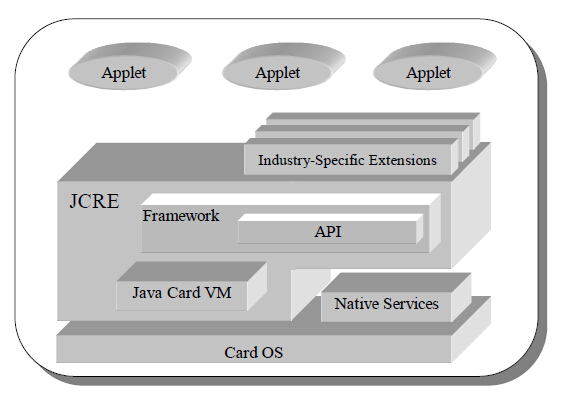
\includegraphics[width=1.2\textwidth]{scc.jpg}
		\caption[ ]{Smart Card Software Components\cite{jcadg}}
	\label{fig:scc}
\end{figure}

\subsubsection{Smart Card Software Components}
As illustrated in figure~\ref{fig:scc}, one typical smart card software includes Card Operation System, native services such as I/O operation and memory management, Java Card Runtime Environment(JCRE) that consists of Java card  Virtual Machine and Framework who is in charge of dispatching APDU as well as applet management, installed applet and at last other optional industry specific extensions\cite{jcadg}

\subsubsection{Data Exchange with Smart Card}
The communication protocol between smart card and terminal is described as Master-Slave relationship\cite{handbuch}, that means terminal device knowns as Master processes unidirectional control over its slave, namely smart card. Once Master-Slave relationship is established, each communication will be initialized by Master and Slave only reacts based on Master's command. 

When a smart card is inserted in a terminal, Master will send its Slave a RESET command which causes smart card to perform a Power-on-Reset behavior. After this Power-on-Reset, smart card informs Master using Answer-to-Rest (ATR) message about card state and communication parameters. In the next step, if necessary terminal will generate a Protocol Type Select (PTS) command, which is used to choose communication protocol and parameters suggested by smart card. After a successful negotiation, smart card and terminal are able to exchange date using Application Protocol Data Unit.
  
Application Protocol Data Unit, or APDU for short, is used  to perform data exchange between smart card and CAD and its structures satisfy ISO 7816-4 specification\cite{chen}. There are two categories of APDU, namely command APDU and response APDU. Command APDU structure and response APDU structure are described in Table~\ref{table:capdu} and Table~\ref{table:rapdu} respectively\cite{handbuch}. 

\begin{table}[!htbp]
\caption{Command APDU Structure}
\centering
\begin{tabular}{ c c c}
\hline\hline
 CLA &class byte identifying application  & mandatory \\[0.5ex]
 INS &instruction byte representing the actual command  & mandatory \\
 P1 &parameter 1 used to provide more command information & mandatory \\
 P2 &parameter 2 used to provide more command information& mandatory \\
 Lc field &the length of data received by card & mandatory \\
 data field &data sent to card& optional \\
Le field &the length of data sent by card \\
\hline
\end{tabular}
\label{table:capdu}
\end{table}

\begin{table}[ht]
\caption{Command APDU Structure}
\centering
\begin{tabular}{ c c c}
\hline\hline
 data field & length decided by Le of preceding command  APDU  & mandatory \\[0.5ex]
 SW1 &state word 1 also called return code 1  & mandatory \\
 SW2 &state word 2 also called return code 2& mandatory \\
\hline
\end{tabular}
\label{table:rapdu}
\end{table}

\subsubsection{Secure Messaging}
Since all communication between smart card and terminal is based on digital electrical pulse performed on card I/O line, attacker can easily record all communication information and and recover it. Therefore secure messaging mechanism is proposed and used to protect against aforementioned message eavesdropping, to ensure authenticity and confidentiality of exchanged information.

In secure message mechanism, both message sender and receiver must agree on to be applied message cryptographic algorithms and corresponding pre-shared keys. In telecommunication domain in accordance with ISO/IEC 7816-4\cite{handbuch}, TLV(Type-lengthl-valuse)-formed data, which encapsulates relative user information, is used to perform secure messaging as data carrier.

\subsection{GlobalPlatform and Remote Application Management}

\begin{figure}[!htbp]
	\centering
	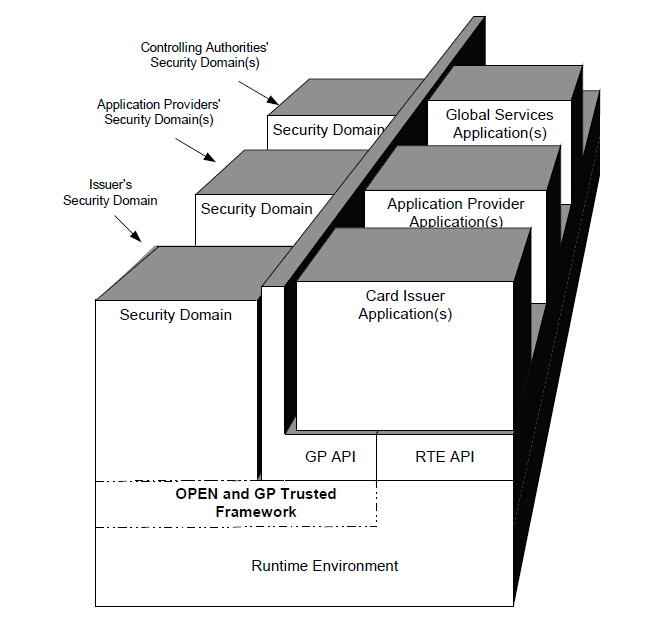
\includegraphics[width=1.2\textwidth]{gp_1.jpg}
		\caption[ ]{Card Operation System Architecture\cite{gp}}
	\label{fig:gp_1}
\end{figure}
GlobalPlatform is an international non-profit organization that provides standardized specifications for multiple smart card applications. It is now widely accepted and used as industry standard for managing Java Applet based application on Javacard Operation System in several domains, for instance in communication industries and payment company\cite{gp}. 

As shown in figure~\ref{fig:gp_1},  the GlobalPlatform card architecture contains four essential parts. The runtime environment, that provides hardware-neutral API for card application  and manages card memory spaces. The on card installed applications, which offers customers various functionalities and services. The security domain (SD), that is usually associated with particular application and known as on-card representatives  of off-card  authorities. SD is in charge of message encryption as well as decryption, creation and validation of digital signature and handling keys used in cryptographic processes. The last component is OPEN framework\cite{gp}.

\subsubsection{OPEN - GlobalPlatform Environment}
OPEN provides various sets of APIs offering functionalities such as entity authentication, remote data exchange, secure channel configuration and remote application management. This framework also performs APDU dispatching as well as is application selection and logical channel management\cite{gp}. Logical channel is designed to enable the data exchange between multi applications and one terminal. Each opened logical channel will handle message regard of one application.  Moreover the special logic channel named basic channel is always opened. In order to ensure system security, OPEN supports secure mechanisms such as,  user authentication , resource availability guarantee and secure channel protocol .
\paragraph{Secure Channel Protocol}
In particular, GlobalPlatform has designed the secure mechanism: secure channel protocol, to guarantee a secure communication. It ensure confidentiality of exchanged information and offers date integrity check.  Moreover Secure Channel Protocol also introduces  a cryptographic exchange process to let smart card and off-card entities to perform entity authentication with each other. 

\subsection{Java Card}
Java Card technology not only adopts the distinguishing features from Java, such as productivity, security and portability\cite{jcadg}, it also makes Java technology available on smart card, where programmer must be faced with more harsh conditions, like limited memory resource and computer ability.

In contrast with Java VM, Java Card VM consists of two parts, the on-card part, which is in charge of bytecode execution, class as well as object management and secure data exchange, the off-card part, which is the real Java Converter.
 \begin{figure}[!htbp]
	\centering
	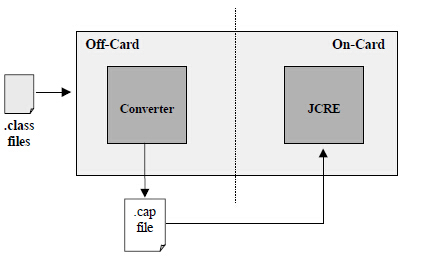
\includegraphics[width=1\textwidth]{jcvm.jpg}
		\caption[ ]{Java Card VM Components\cite{jcadg}}
	\label{fig:jcvm}
\end{figure}
As illustrated in figure~\ref{fig:jcvm}, a complied Java applet (.cap file) is generated by off-card Converter based on inputed Java class file and executed by on-card Java Card Runtime Environment (JCRE). 

\subsubsection{Language Specification}
Apart from above mentioned Java Card VM, compared with original Java language, Java card has many unique features.
Since current smart card does not support multitasking, therefore threads are not backed up in Java Card. Also garbage collection  is performed by VM, as a result function \emph{finalize()} is not supported. Moreover because on smart card, memory space and process ability is limited, as a result programmer can only use three main primitive types, namely byte, short and boolean. Furthermore only one-dimensional array is offered. Nonetheless Java card language supports all features of inheritance and provides all Java language security features, for example, private access modifiers as well as bytecode verification\cite{jcadg}.

\subsubsection{Transaction Integrity}
One of the most import features of Java Card technology is that Java Card Runtime Environment ensures the integrity of transaction, which means even an unexpected loss of power occurs on smart card, the ongoing transactions' integrity is protected with the help of following schema\cite{handbuch}:
\begin{verbatim}
// Transaction Starts
JCSystem.beginTranscation();

doSomething

//Transaction Ends
JCSystem.commitTransaction();
\end{verbatim}
Only when JCRE finishes running method \emph{JCSystem.commitTranscation()}, the corresponding transaction will be finished and submitted. Otherwise JCRE will throw transaction exception and reset data that involved in this broken transaction.

\subsubsection{Persistent Object and Transient Object}
In  the realm of Java Card, all objects are preserved in nonvolatile memory, which means this persistent object exits on smart card beyond the execution time of corresponding applet, as long as there exits a reference pointing to it. But also it is allowed to develop transient object on Java card. To be precisely, for instance class array object stays in nonvolatile memory space but in contrast one actual instance of array in stored in volatile memory\cite{handbuch}.
\subsubsection{Java Card Applet}
Java Card Applet refers to the Java Card language programmed code, which extends the class \emph{Applet} from package \emph{javacard.framework}. Meanwhile Java Card Applet should implement following four methods:
\begin{itemize}
\item\emph{install()}, this method must be implemented and be used to create an applet instance.
\item\emph{process(APDU)}, the implementation of this method is also mandatory and uses APDU as input parameter. In this method applet developer designs how to process APDU sent to this applet and which APDU response should be generated.
\item \emph{select()}, when JCRE detects a SELECT APDU command, which is applied to select one installed applet, JCRE will call this method of to be selected applet.
\item  \emph{deselect()}, this method is called by JCRE to inform corresponding applet that it is no longer selected by JCRE.
\end{itemize}

After finishing programming one Applet, it comes to next phase, namely applet installation. This process takes place usually at the factory or office under the control of card issuer. When one applet is installed on smart card, it only directly communicates with JCRE and other installed applet classes. It should be pointed out, this installed Java Card applet is also belongs to \emph{persistent object} and stored in smart card nonvolatile memory space. Every Java Card Applet is assigned one unique Application ID, which is also known as AID and be used by JCRE to \emph{register} and \emph{select} corresponding applet at run time.

\subsubsection{Javacard Cryptography}
Javacard provides a list of APIs to support not only smart card application and data exchange security but also to reinforce other system's security by acting as essential security token. 
In order to ensure sure messaging between smart card and terminal following three aspects must be considered:
\begin{itemize}
\item \emph{Entity Authentication:} Usually mutual authentication is applied to guarantee the authorities of both communication partners.
\item \emph{Message Confidentiality:} The transfered information is encrypted using algorithms negotiated between two communication entities to ensure data privacy and security.
\item \emph{Message Integrity:} In order to protect exchanged message from unauthorized modification and to provide authenticity assurance, message authentication code (MAC) is calculated based on to be transfered data and integrated in that message.
\end{itemize}
Packages \emph{javacard.security} and \emph{javacardx.crypto} support aforementioned security mechanism with following class and interfaces\cite{chen}:

\begin{table}[ht]
\caption{package: \emph{javacard.security}}
\centering
\begin{tabular}{lllll}
\hline
 Class or Interface & Function Description\\
\hline\hline
 Key &Interface for all keys   \\
 SecrectKey &Interface for symmetric algorithms' keys\\
DESKey & Interface for keys used for DES or two-key triple DES or three-key triple DES\\
PrivateKey &Interface for private keys\\
PublicKey & Interface for public keys\\
RSAPrivateKey& Interface for keys used by RSA algorithm to sign data\\
RSAPublicKey & Interface for keys used to verify signatures generated with RSA \\
DSAKey& Interface for keys used by DSA\\ 
DSAPrivateKey& Interface for keys to sign data with DSA algorithm\\
DSAPublicKey& Interface for keys to verify signatures generated with DSA\\
KeyBuilder& Factory class implemented to construct key objects\\
MessageDigest& Abstract class for hashing algorithm\\
Signature& Abstract class for signature algorithm\\
RandomData&Abstract class for generation of random data \\
CrptoException& Exception class\\
\hline
\end{tabular}
\label{table:rapdu}
\end{table}

\begin{table}[ht]
\caption{package: \emph{javacardx.crypto}}
\centering
\begin{tabular}{lllll}
\hline
 Class or Interface & Function Description\\
\hline\hline
Cipher & Abstract class offers cryptographic cipher used for encryption and decryption\\
KeyEncryption & Class provides implementation of keys\\
\hline
\end{tabular}
\label{table:rapdu}
\end{table}


\subsection{Android}

\section{State of Art}
\section{Implementation Scenario}
 \begin{figure}[!htbp]
	\centering
	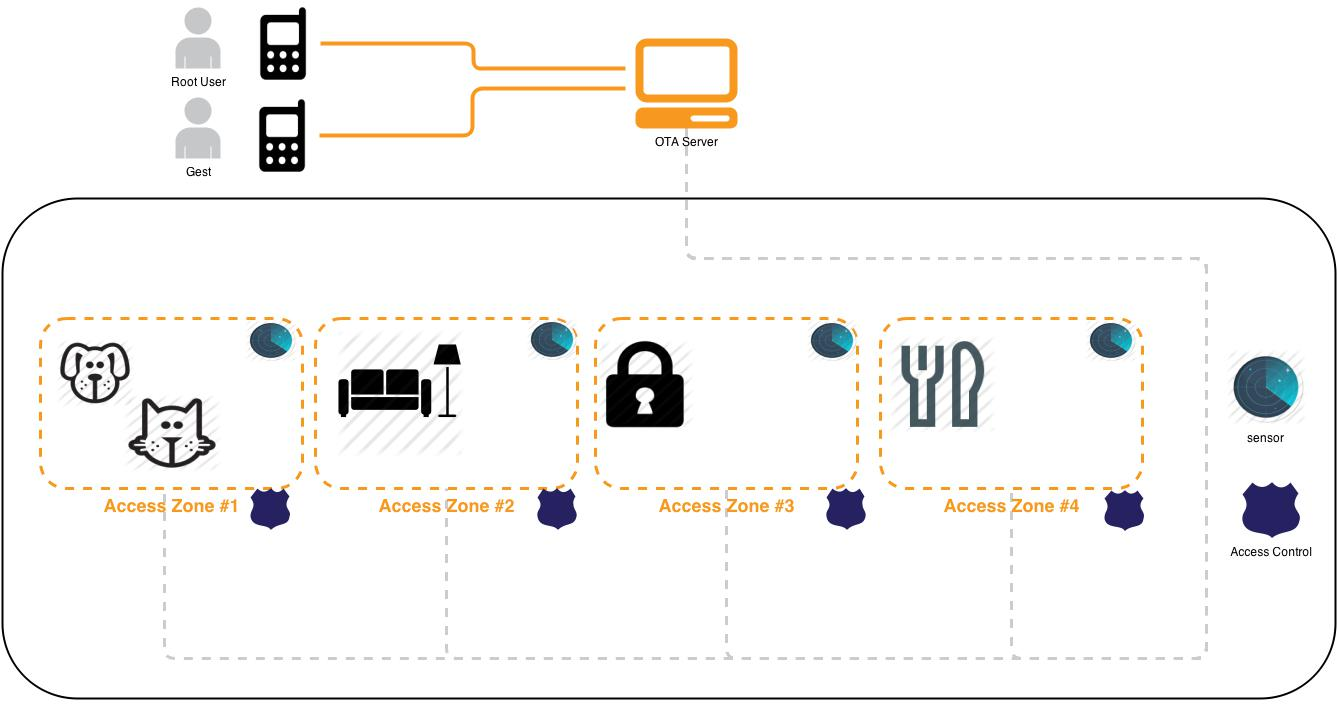
\includegraphics[width=1.2\textwidth]{homeoverview.jpg}
		\caption[ ]{Smart Home}
	\label{fig:SmartHome}
\end{figure}
\subsection{Overview}
Figure~\ref{fig:SmartHome} describes the basic structure and functionalities provided by implementation scenario-Smart Home.
In each room , embedded with UICC smart card sensors which are in charge of monitoring environment variables, such as, home temperature, luminance and how much water the pet has, as well as embedded UICC smart card device controller whose responsibility is to control electric devices based on user's commands, such as opening windows, turning off the heating or starting to make coffee, are deployed. On each those sensor and control device an OPC UA server is installed, its major responsibility is controlling that corresponding device as well as data gathered by it.  Moreover each door in this scenario is equipped with a digital lock, that only allows people with enough authority to access. Also a OPC UA server exists on those locks and they are embedded with UICC smart card. Users in this scenario can be home owner or guests. Using embedded with UICC smart card cell phone and on this mobile terminal installed OPC UA client application, subscriber is capable of configuring sensor and control device , remote controlling aforementioned secure devices, viewing historical information recorded by corresponding facilities. With the help of such services a comfortable living condition is created in an automated way.  Moreover the root user, namely the owner of this house, is also able to assign the permission of accessing particular room to other guests. In case of when he/she is taking a vocation and pet cannot get necessary care.


In this implementation scenario, OPC UA clients, namely Universal Integrated Circuit Card (UICC)  based phone user communicates with OPC UA server, which is deployed on other secure hard devices, via an OTA server.   Smart card that is applied in this scenario acts as security token for both OPC UA client and server and it contains credential information like encryption keys. certificates and digital signature. The communication stack, that manages secure  communication between OPC UA client and server application, is also developed and integrated on smart card as a Java Card applet, which means without corresponding UICC card, OPC UA client and server are not able to appropriately finish their work.
 \begin{figure}[ht]

	\centering
	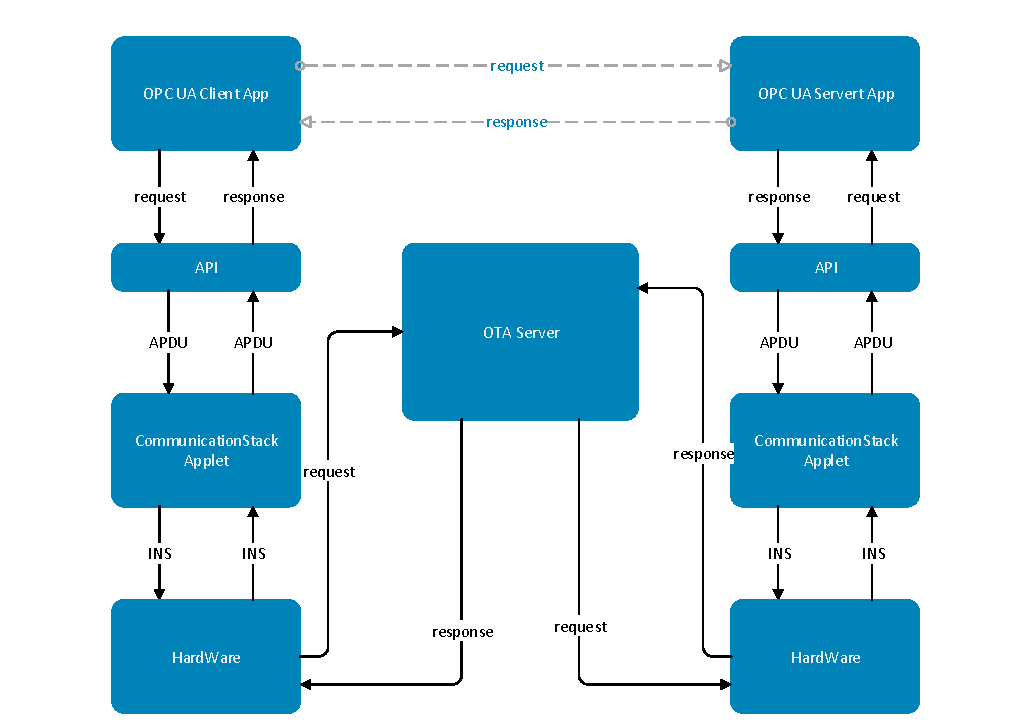
\includegraphics[width=1.1\textwidth]{csoverview}
		\caption[ ]{OPC UA Client Server Structure}
	\label{fig:softwareStructure}
\end{figure}


\subsection {Software Structure}
Figure~\ref{fig:softwareStructure} pictures aforementioned OPC UA client server structure. OP UA Client and Server application communicate with each other with the help of an OTA server. And the communication stack,  is in charge of creation and managing the secure communication between OTA server and secure device. Moreover using different chip card, OPC UA client application is able to communicate with OPC UA server application using Short Message Service(SMS) or TCP/IP based web service. 
\newline
server on secure device provides following services:
 \begin{itemize}
  \item processing client subscription/publishing environment data
  \item secure message exchange with client
  \item authority management
  \item historical data record
  \item execution client's command
\end{itemize}
Basic client functions as following are provided:
 \begin{itemize}
  \item submitting subscription/receiving published data
  \item secure message exchange with server
  \item sending command/configuration data
  \item providing user friendly interface
\end{itemize}

Communication stack is integrated  in UICC smart card, whose responsibility is realizing secure channel as well as session management, transporting data to receiver using TCP/IP connections. An internal API translates OPC UA application instructions in to Application Protocol Data Unity (APDU) messagse and forwards them to smart card OS, which is eventually in charge of user authentication and processing secure messaging between card application and chip card pair. 

Moreover thanks to self-containment structure, smart card itself does not dependent on other external resources, which could be extreme vulnerable to potential secure attack, and therefore provides a better hardware security and OS security.

 \begin{figure}
	\centering
	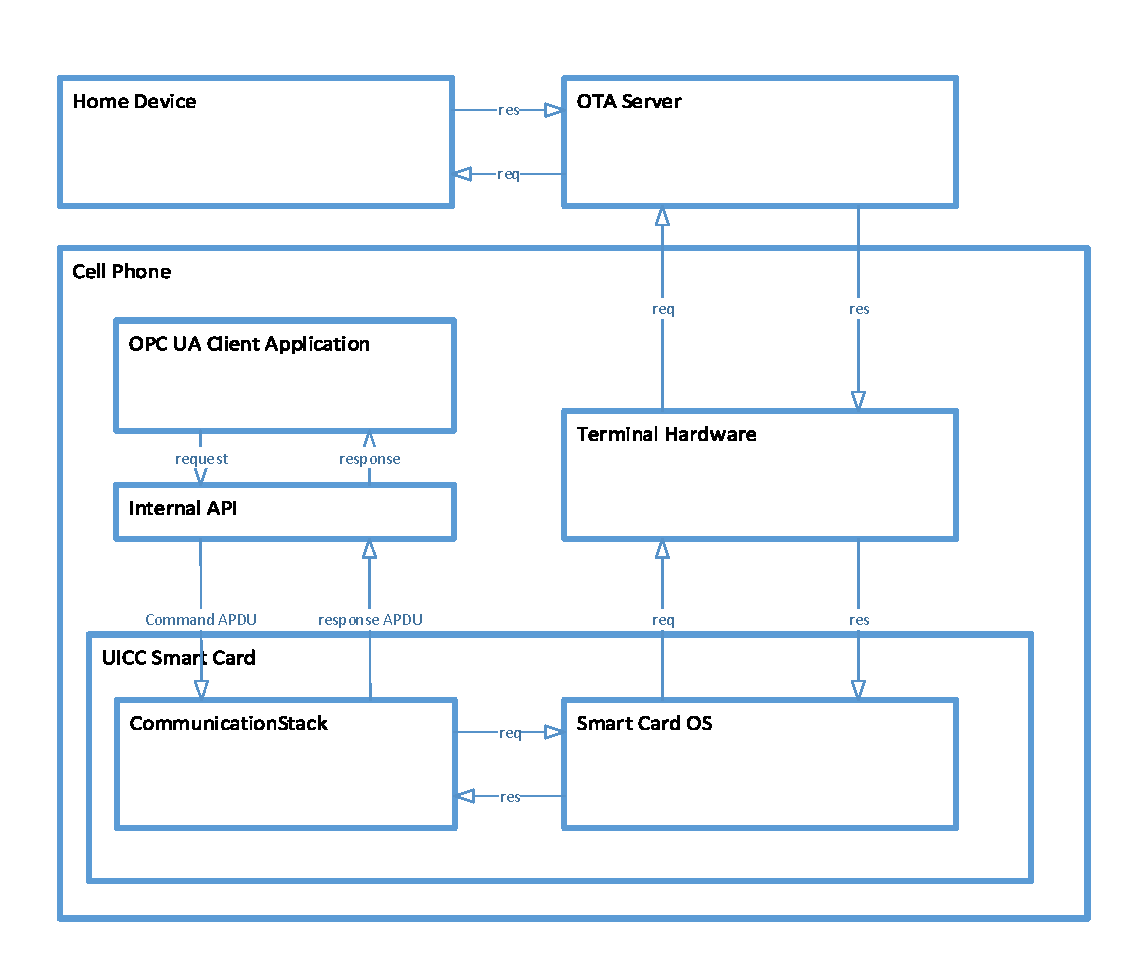
\includegraphics[width=1.0\textwidth]{clientStructure}
		\caption[ ]{Client Structure}
	\label{fig:clientStructure}
\end{figure}
\subsubsection{Client Structure}
As described in figure~\ref{fig:clientStructure}, the OPC UA client consists of client application code that realizes client application level functions, OPC UA client API that translates client application instructions into APDU and forwards APDU to UICC smart card. The Communication stack is developed and integrated with UICC card, which is in charge of creation and management TCP/IP connection, secure channel between client and server. This communication stack is based on card OS components provided by Global Platform. 
\begin{figure}
	\centering
	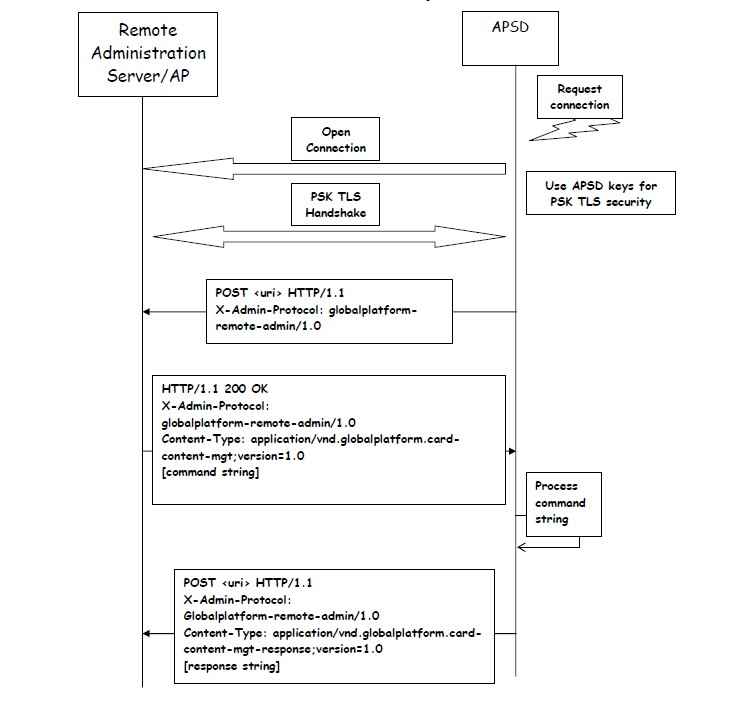
\includegraphics[width=1.2\textwidth]{apsd.jpg}
		\caption[ ]{Communication Flow between an AP and corresponding APSD\cite{ramGP}}
	\label{fig:apsd}
\end{figure}
Global Platform provides and defines communication flow between an application provider and smart card, allows information exchanged between a remote entity and a terminal, this process is also known as  Remote Application Management(RAM) based on HTTP protocol and PSK TLS security Over-the-Air. The on card component, which is responsible for connection creation with the remote entity and user/application authentication, is called Security Domain. And the aforementioned remote entity  is  referred as Remote Administration Server as well. With these concepts, smart card with Security Domain issued  by GloablPlatform can act as HTTP client and is capable of packing APDU formate information into HTTP POST message and transmitting HTTP message to OTA server. At the same time, the Remote Administration Server also is a HTTP server, which can send HTTP message including APDU format information to its client.\cite{ramGP}
 
Figure~\ref{fig:apsd} illustrates a typical communication flow between administration server and corresponding security domain (Application Security Domain) on smart card. As can be seen, the request for open communication is alway initialized by security domain, which is also the phone user. After a successful creation of secure handshake, the remote administration server and security domain is able to use HTTP message to exchange request and response strings, which include APDU instructions. GlobalPlatform has also provided  a lists of API used to initialize authentication process, to configure algorithm and keys for message  encryption and decryption, to perform message exchange  behavior and so on.

\subsubsection{Server Structure}

\begin{figure}
	\centering
	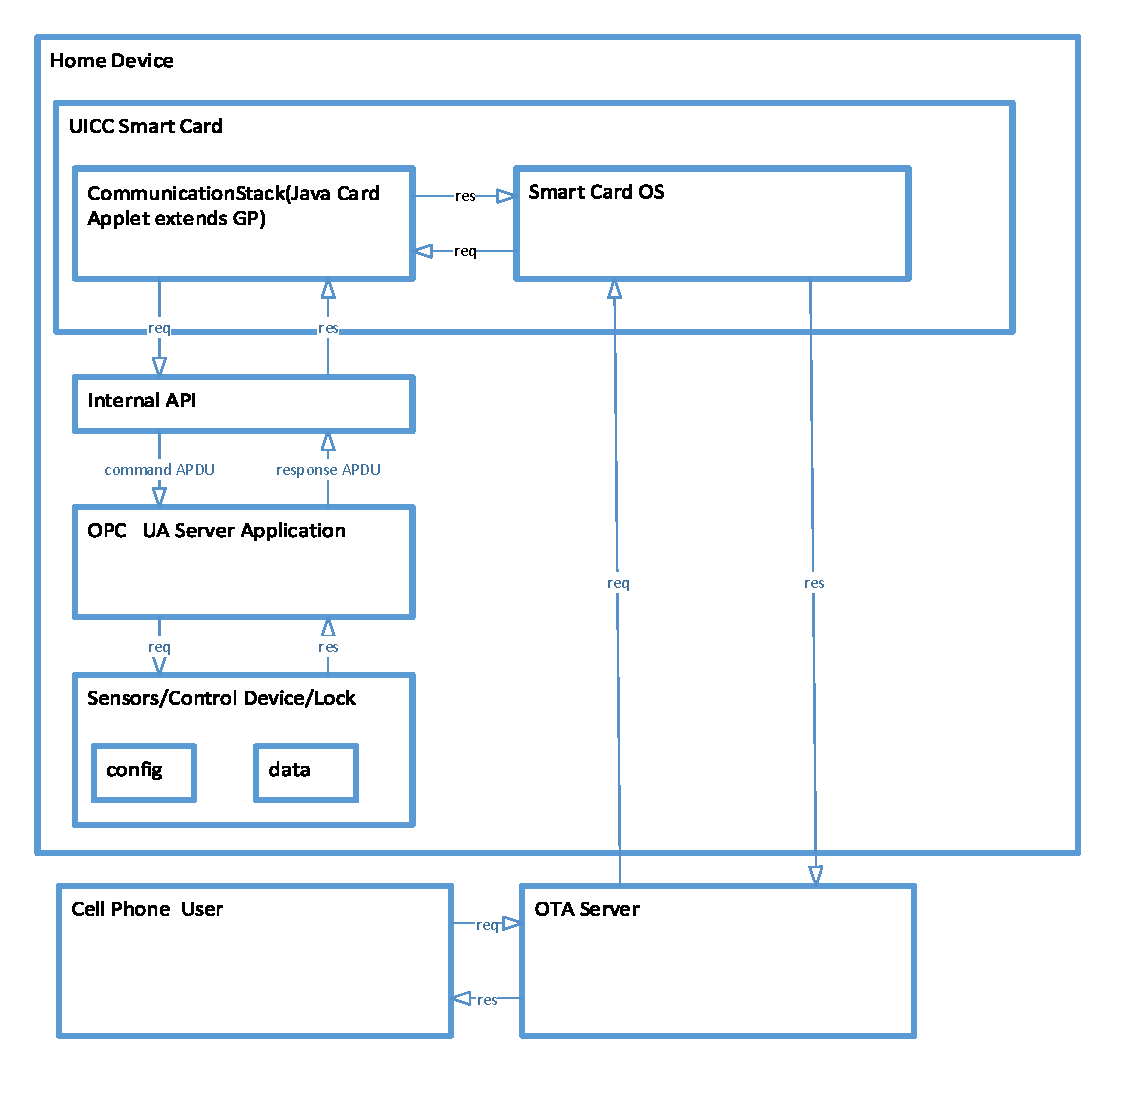
\includegraphics[width=0.9\textwidth]{serverStructure}
		\caption[ ]{Server Structure}
	\label{fig:serverStructure}
\end{figure}
Server here refers sensors, control device as well digital locks that together build up the smart home system. Each server controls exactly one above-mentioned secure device and take subscription as well as publish corresponding notification to authenticated subscriber. The server structure is pictured as figure~\ref{fig:serverStructure} and it consists of OPC UA server application code, which offers basic server like subscription and notification mentioned before, an internal API, that translate OPC UA instructions into APDU, and a on smart card integrated communication stack, that is responsible for user authentication, secure message exchange and so on.

\subsubsection{Implementation Tool Support}
Morpho presents JACADE with full name, Java Card Applet Develop Environment, which is more than just a IDE but a complex selection of various class API and software modules, that can be applied to design complete Java Card Applet as well as to debug Java source. When it comes to running test with Java Card Applet, apart from using regular cell phone with UICC smart card, on where to be tested applet is installed, Morpho Card Reader (MCR) or Java virtual card together with iCardReader, Universal Test Environment (UTE) can be applied. To be more specifically, iCardReader is a tool developed by Morpho and be used in order to send APDU script to Java virtual card or to real smart card connected with test PC using smart card reader such as MCR reader, and to monitor corresponding response APDU information. Universal Test Environment provided by Morpho uses Java languages developed test cases and test scenarios\footnote{Test scenario is a collection of relative test cases.} to simulate user cases and obverse related smart card reactions. In contrast with iCardreader, which can only send APDU command sequence to smart card, UTE integrates more software models that can be used to simulate such as security domain offered by other card application provider, and therefore can provide more sophisticate test environment.
\section{System Design}
\subsection{Communication Applet Design}
\subsubsection {Interface between Applet and CAD}
Before concrete implementation of Javacard Applet code, the interface, which in essence is a set of commond APDUs and corresponding response APDUs, between applet and CAD must be well defined.  The CommunicationStack support two categories commond APDU:
 \begin{itemize}
  \item The \emph{SELECT} Command APDU, which is used by JCRE to select CommunicationStack applet.
  \item Other command APDUs, which are introduced in order to provide functionalists such as: entity authentication, message exchange as well as cipher negotiation and etc.
\end{itemize}

\paragraph{SELECT APDU}
The header of this command APDU is fixed and \emph{Lc} indicates the length of CommunicationStack AID. In\emph{Data filed} real AID is saved.
\begin{table}[h]
\caption{SELECT command APDU}
\resizebox{\textwidth}{!}{%
\begin{tabular}{|l|l|l|l|l|l|l|}
\hline
CLA  & INS  & P1   & P2   & Lc   & Data field                                                                                          & Le  \\ \hline
0x00 & 0xA4 & 0x04 & 0x00 & 0x0A & \begin{tabular}[c]{@{}l@{}}0x00, 0x01, 0x02, 0x03, 0x04\\ 0x05, 0x06, 0x07, 0x08, 0x09\end{tabular} & N/A \\ \hline
\end{tabular}
}
\label{select-apdu}
\end{table}
Two categories of response APDUs are expected, one represents successful processing of \emph{SELECT} command APDU and the other stands for failure.
\begin{table}[h]
\caption{SELECT response APDU}
\label{select-response-apdu}
\resizebox{\textwidth}{!}{%
\begin{tabular}{|l|l|l|}
\hline
Optional data & Status word & Description                                \\ \hline
No data       & 0x9000      & Successful processing                      \\ \hline
              & 0x6999      & Failed to select CommunicationStack applet \\ \hline               
\end{tabular}
}
\end{table}

\paragraph{Entity Authentication}
When CommunicationStack is successfully select by JCRE, it then comes to entity authentication phase, which consist of authentication process between UICC and OTA server as well as authentication process between UICC and OPC UA application code.
\bibliography{opc_ua}
\bibliographystyle{splncs}

\end{document}
